\documentclass[final,a1paper]{baposter}
%\documentclass[a4shrink,portrait,final]{baposter}
% Usa a4shrink for an a4 sized paper.

\tracingstats=2

\usepackage{times}
\usepackage{calc}
\usepackage{graphicx}
\usepackage{amsmath}
\usepackage{amssymb}
\usepackage{relsize}
\usepackage{multirow}
\usepackage{bm}

\usepackage{harvard}
\citationmode{abbr} % forces use of et al all the time (normally only after first one is full cite)
\renewcommand{\refname}{} % removes the auto inserted "References" header

% This sets the default font to be sans serif
\renewcommand{\familydefault}{\sfdefault}

\usepackage{graphicx}
\usepackage{multicol}

\pgfdeclarelayer{background}
\pgfdeclarelayer{foreground}
\pgfsetlayers{background,main,foreground}

\usepackage{helvet}
%\usepackage{bookman}
\usepackage{palatino}

% Added by Louis
\usepackage{wrapfig}
\usepackage{enumerate}
\usepackage{float}
\usepackage{arydshln} % for dashed lines
\linespread{1.2}
% End added by Louis

\newcommand{\captionfont}{\footnotesize}

\selectcolormodel{cmyk}

\graphicspath{{images/}}

%%%%%%%%%%%%%%%%%%%%%%%%%%%%%%%%%%%%%%%%%%%%%%%%%%%%%%%%%%%%%%%%%%%%%%%%%%%%%%%%
%%%% Some math symbols used in the text
%%%%%%%%%%%%%%%%%%%%%%%%%%%%%%%%%%%%%%%%%%%%%%%%%%%%%%%%%%%%%%%%%%%%%%%%%%%%%%%%
% Format 
\newcommand{\Matrix}[1]{\begin{bmatrix} #1 \end{bmatrix}}
\newcommand{\Vector}[1]{\Matrix{#1}}
\newcommand*{\SET}[1]  {\ensuremath{\mathcal{#1}}}
\newcommand*{\MAT}[1]  {\ensuremath{\mathbf{#1}}}
\newcommand*{\VEC}[1]  {\ensuremath{\bm{#1}}}
\newcommand*{\CONST}[1]{\ensuremath{\mathit{#1}}}
\newcommand*{\norm}[1]{\mathopen\| #1 \mathclose\|}% use instead of $\|x\|$
\newcommand*{\abs}[1]{\mathopen| #1 \mathclose|}% use instead of $\|x\|$
\newcommand*{\absLR}[1]{\left| #1 \right|}% use instead of $\|x\|$

\def\norm#1{\mathopen\| #1 \mathclose\|}% use instead of $\|x\|$
\newcommand{\normLR}[1]{\left\| #1 \right\|}% use instead of $\|x\|$

%%%%%%%%%%%%%%%%%%%%%%%%%%%%%%%%%%%%%%%%%%%%%%%%%%%%%%%%%%%%%%%%%%%%%%%%%%%%%%%%
% Multicol Settings
%%%%%%%%%%%%%%%%%%%%%%%%%%%%%%%%%%%%%%%%%%%%%%%%%%%%%%%%%%%%%%%%%%%%%%%%%%%%%%%%
\setlength{\columnsep}{0.7em}
\setlength{\columnseprule}{0mm}


%%%%%%%%%%%%%%%%%%%%%%%%%%%%%%%%%%%%%%%%%%%%%%%%%%%%%%%%%%%%%%%%%%%%%%%%%%%%%%%%
% Save space in lists. Use this after the opening of the list
%%%%%%%%%%%%%%%%%%%%%%%%%%%%%%%%%%%%%%%%%%%%%%%%%%%%%%%%%%%%%%%%%%%%%%%%%%%%%%%%
\newcommand{\compresslist}{%
\setlength{\itemsep}{1pt}%
\setlength{\parskip}{0pt}%
\setlength{\parsep}{0pt}%
}


%%%%%%%%%%%%%%%%%%%%%%%%%%%%%%%%%%%%%%%%%%%%%%%%%%%%%%%%%%%%%%%%%%%%%%%%%%%%%%
%%% Begin of Document
%%%%%%%%%%%%%%%%%%%%%%%%%%%%%%%%%%%%%%%%%%%%%%%%%%%%%%%%%%%%%%%%%%%%%%%%%%%%%%

\begin{document}

%%%%%%%%%%%%%%%%%%%%%%%%%%%%%%%%%%%%%%%%%%%%%%%%%%%%%%%%%%%%%%%%%%%%%%%%%%%%%%
%%% Here starts the poster
%%%---------------------------------------------------------------------------
%%% Format it to your taste with the options
%%%%%%%%%%%%%%%%%%%%%%%%%%%%%%%%%%%%%%%%%%%%%%%%%%%%%%%%%%%%%%%%%%%%%%%%%%%%%%
% Define some colors
\definecolor{silver}{cmyk}{0,0,0,0.3}
\definecolor{yellow}{cmyk}{0,0,0.9,0.0}
\definecolor{reddishyellow}{cmyk}{0,0.22,1.0,0.0}
\definecolor{black}{cmyk}{0,0,0.0,1.0}
\definecolor{darkYellow}{cmyk}{0,0,1.0,0.5}
\definecolor{darkSilver}{cmyk}{0,0,0,0.1}

\definecolor{lightyellow}{cmyk}{0,0,0.3,0.0}
\definecolor{lighteryellow}{cmyk}{0,0,0.1,0.0}
\definecolor{lighteryellow}{cmyk}{0,0,0.1,0.0}
\definecolor{lightestyellow}{cmyk}{0,0,0.05,0.0}

\definecolor{tcdblue}{RGB}{0,114,198} % This is the officially recognised TCD blue, as defined on the TCD website
\definecolor{tcdgrey}{RGB}{83,86,90}  % This is the officially recognised TCD grey, as defined on the TCD website


%%
\typeout{Poster Starts}
\background{
  \begin{tikzpicture}[remember picture,overlay]%
    \draw (current page.north west)+(-2em,2em) node[anchor=north west] {\includegraphics[height=1.1\textheight]{silhouettes_background}};
  \end{tikzpicture}%
}

\newlength{\leftimgwidth}
\begin{poster}%
  % Poster Options
  {
  % Show grid to help with alignment
  grid=no,
  % Column spacing
  colspacing=1em,
  % Color style
  bgColorOne=white,
  bgColorTwo=white,
  borderColor=tcdblue,
  headerColorOne=white,
  headerColorTwo=white,
  headerFontColor=tcdblue,
  boxColorOne=white,
  boxColorTwo=white,
  % Format of textbox
  textborder=roundedleft,
  % Format of text header
  eyecatcher=no,
  headerborder=open,
  headerheight=11em, %0.12\textheight,
  headershape=roundedright,
  headershade=plain,
  headerfont=\Large,
  boxshade=plain,
%  background=shade-tb,
  background=plain,
  linewidth=1pt
  }
  % Eye Catcher
  {
\includegraphics[height=7em]{trinity-common-use.jpg}} % No eye catcher for this poster. (eyecatcher=no above). If an eye catcher is present, the title is centered between eye-catcher and logo.
  % Title
  {{\huge Networks with Redundant Subsystems}\\{\LARGE Faster Inference for Phase-type Distributions}}
  % Authors
  {
  
  \vspace{-1.5em}
  Louis JM Aslett {\smaller (louis@maths.tcd.ie)} and Simon P Wilson {\smaller (swilson@tcd.ie)}
  
  \vspace{0.2em}
  Trinity College Dublin
  }
  % University and sponsor logos
  {
      \begin{minipage}{19em}
       \hfill
        
\includegraphics[height=5.5em]{trinity-stacked.jpg}
        % \hfill
        % 
\includegraphics[height=9em]{IRCSETlogo}
        
\includegraphics[height=5.5em]{SFI_logo_stacked_en.jpg}
         % \hfill
      \end{minipage}
  }

  \tikzstyle{light shaded}=[top color=baposterBGtwo!30!white,bottom color=baposterBGone!30!white,shading=axis,shading angle=30]

  % Width of left inset image
     \setlength{\leftimgwidth}{0.78em+8.0em}

%%%%%%%%%%%%%%%%%%%%%%%%%%%%%%%%%%%%%%%%%%%%%%%%%%%%%%%%%%%%%%%%%%%%%%%%%%%%%%
%%% Now define the boxes that make up the poster
%%%---------------------------------------------------------------------------
%%% Each box has a name and can be placed absolutely or relatively.
%%% The only inconvenience is that you can only specify a relative position 
%%% towards an already declared box. So if you have a box attached to the 
%%% bottom, one to the top and a third one which should be in between, you 
%%% have to specify the top and bottom boxes before you specify the middle 
%%% box.
%%%%%%%%%%%%%%%%%%%%%%%%%%%%%%%%%%%%%%%%%%%%%%%%%%%%%%%%%%%%%%%%%%%%%%%%%%%%%%
    %
    % A coloured circle useful as a bullet with an adjustably strong filling
    \newcommand{\colouredcircle}[1]{%
      \tikz{\useasboundingbox (-0.2em,-0.32em) rectangle(0.2em,0.32em); \draw[draw=black,fill=baposterBGone!80!black!#1!white,line width=0.03em] (0,0) circle(0.18em);}}




%%%%%%%%%%%%%%%%%%%%%%%%%%%%%%%%%%%%%%%%%%%%%%%%%%%%%%%%%%%%%%%%%%%%%%%%%%%%%%
\headerbox{1. The Problem}{name=the_problem,column=0,row=0}{
%%%%%%%%%%%%%%%%%%%%%%%%%%%%%%%%%%%%%%%%%%%%%%%%%%%%%%%%%%%%%%%%%%%%%%%%%%%%%%
	Phase-type (PHT) distributions are a natural choice for modelling the multiple phases
	of failure and repair which a redundant subsystem may go through before ultimately becoming
	unavailable.
	
	\vspace{0.5em}
	\citeasnoun{bladt2001} present a scheme for Bayesian inference on general PHT distributions.
	There are some key areas where there is scope to extend this work in a reliability context:
	\begin{enumerate}[i)]
		\item the need to account for censoring and other common situations in reliability;
		\item the need for parameter constraints;
		\item the sampling scheme is intractably slow for the PHT distributions commonly encountered in reliability.
	\end{enumerate}
}

%%%%%%%%%%%%%%%%%%%%%%%%%%%%%%%%%%%%%%%%%%%%%%%%%%%%%%%%%%%%%%%%%%%%%%%%%%%%%%
  \headerbox{References}{name=refs,column=0,span=2,above=bottom}{
%%%%%%%%%%%%%%%%%%%%%%%%%%%%%%%%%%%%%%%%%%%%%%%%%%%%%%%%%%%%%%%%%%%%%%%%%%%%%%
	\vspace{-2em}
	% Put here your bibtex stuff:
	\bibliographystyle{agsm}
	\bibliography{Transfer_Report}
}

  
%%%%%%%%%%%%%%%%%%%%%%%%%%%%%%%%%%%%%%%%%%%%%%%%%%%%%%%%%%%%%%%%%%%%%%%%%%%%%%
  \headerbox{2. PHT Distributions}{name=pht,column=0,span=1,below=the_problem,above=refs}{
%%%%%%%%%%%%%%%%%%%%%%%%%%%%%%%%%%%%%%%%%%%%%%%%%%%%%%%%%%%%%%%%%%%%%%%%%%%%%%
	Consider a Continuous-Time Markov Chain (CTMC) with an absorbing state.  Without loss of generality, let the CTMC generator be written:
		\[ \mathbf{T} = \left(\begin{array}{cc}\mathbf{S} & \mathbf{s} \\\mathbf{0}^\mathrm{T} & 0\end{array}\right) \]
		Then, if $X$ is the random variable denoting time to entering the absorbing state:
		\[ \begin{array}{rcl}
			F_X(x) &=& 1 - \boldsymbol{\pi}^\mathrm{T} \exp\{x \mathbf{S}\} \mathbf{e}, \ \ \mathbf{e}=(1, \dots, 1)^\mathrm{T}\\
			f_X(x) &=& \boldsymbol{\pi}^\mathrm{T} \exp\{x \mathbf{S}\} \mathbf{s}
		\end{array} \]
				
		\vspace{0.5em}
		\textbf{Simplest Example:} Consider a dual redundant hot-swappable power supply (PS) subsystem.
		\vspace{-0.5em}
		\begin{center}
			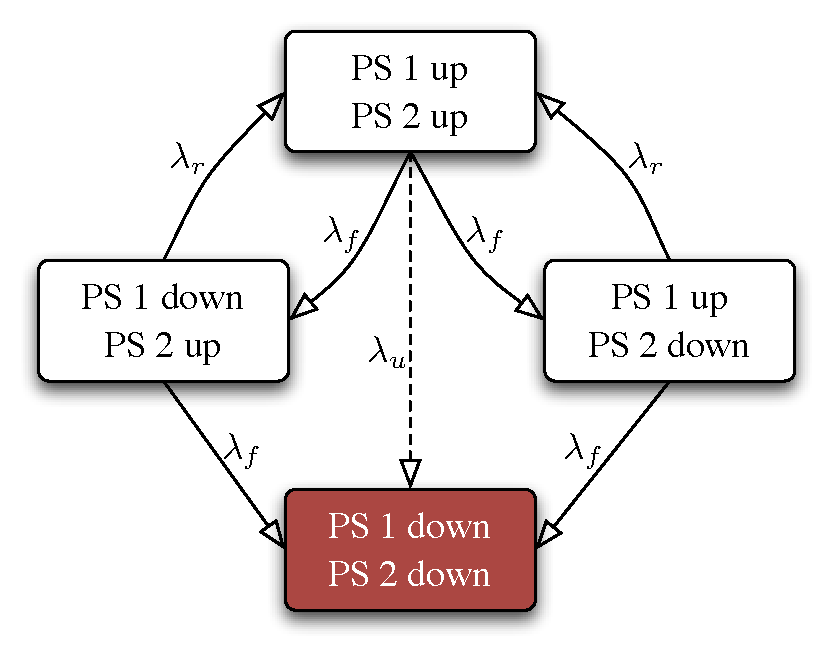
\includegraphics[width=1\textwidth]{CTMC}
		\end{center}
		\vspace{-1em}
		$\lambda_r$ : Repair rate; $\lambda_f$ : Failure Rate; $\lambda_u$ : Uncovered Failure Rate (ignore for simple case).
		\[ \implies \mathbf{T} = 
			\left(\begin{array}{cccc}
				-2\lambda_\mathrm{f} & \lambda_\mathrm{f} & \lambda_\mathrm{f} & 0 \\
				\lambda_\mathrm{r} & -\lambda_\mathrm{r}-\lambda_\mathrm{f} & 0 & \lambda_\mathrm{f} \\
				\lambda_\mathrm{r} & 0 & -\lambda_\mathrm{r}-\lambda_\mathrm{f} & \lambda_\mathrm{f} \\
				0 & 0 & 0 & 0
			\end{array}\right) \]
	% \vspace{0.5em}
}

%%%%%%%%%%%%%%%%%%%%%%%%%%%%%%%%%%%%%%%%%%%%%%%%%%%%%%%%%%%%%%%%%%%%%%%%%%%%%%
\headerbox{Funding}{name=funding,column=2,span=1,above=bottom,below=pht}{
%%%%%%%%%%%%%%%%%%%%%%%%%%%%%%%%%%%%%%%%%%%%%%%%%%%%%%%%%%%%%%%%%%%%%%%%%%%%%%
	\begin{center}
		This work was funded by Science Foundation Ireland under the xxxxx project, grant number xx/xx/xxxxx.
	\end{center}
}


%%%%%%%%%%%%%%%%%%%%%%%%%%%%%%%%%%%%%%%%%%%%%%%%%%%%%%%%%%%%%%%%%%%%%%%%%%%%%%
\headerbox{3. The Algorithm}{name=bladt,column=1,row=0,span=1,above=pht}{
%%%%%%%%%%%%%%%%%%%%%%%%%%%%%%%%%%%%%%%%%%%%%%%%%%%%%%%%%%%%%%%%%%%%%%%%%%%%%%
		Full stochastic process to absorption observed
		
		$\implies\exists$ conjugate priors $\boldsymbol{\pi} \sim \mathrm{Dir}; S_{ij}, s_i \sim \mathrm{Gam}$
				
		\vspace{0.5em}
		\citeasnoun{bladt2001} proposed a Metropolis-Hastings (MH) within Gibbs sampler for the unobserved process case.
		\vspace{-0.5em}
		\begin{itemize}
			\item MH proposal is draw from:
				\vspace{-0.7em}
				\[p(\mathrm{path\ \cdot} \,|\, \boldsymbol{\pi}, \mathbf{S}, Y \ge y_i)\]
				
				\vspace{-1.2em}
				by rejection sampling.
				
				Acceptance ratio $\implies$ last sample from
				\vspace{-0.6em}
				\[p(\mathrm{path\ \cdot} \,|\, \boldsymbol{\pi}, \mathbf{S}, Y = y_i)\]
				
				\vspace{-1.2em}
				after truncating to $y_i$.
				
				\vspace{-1em}
		 	\item sample from unobserved process in MH step gives conjugacy for Gibbs step.
		\end{itemize}
		\vspace{-1.2em}
		\begin{center}
			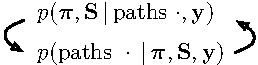
\includegraphics[width=0.55\textwidth]{GibbsStep}
		\end{center}	
	\vspace{0.3em}
}

%%%%%%%%%%%%%%%%%%%%%%%%%%%%%%%%%%%%%%%%%%%%%%%%%%%%%%%%%%%%%%%%%%%%%%%%%%%%%%
\headerbox{4. Censoring/Constraints}{name=cc,column=2,row=0,span=1,above=pht}{
%%%%%%%%%%%%%%%%%%%%%%%%%%%%%%%%%%%%%%%%%%%%%%%%%%%%%%%%%%%%%%%%%%%%%%%%%%%%%%
	%\setlength{\columnsep}{1.5em}
	%\begin{multicols}{2}
		\textbf{Censoring:} arises through competing risks:
		\begin{center}
			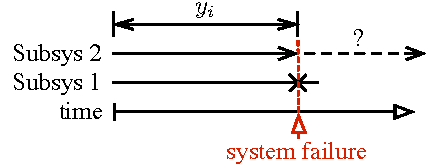
\includegraphics[width=0.8\textwidth]{CompRisks}
		\end{center}
		
		\vspace{-1em}
		Elegantly dealt with by performing just rejection sampling part of MH step.
	%\end{multicols}	
		
		\vspace{0.5em}
		\textbf{Parameter Constraints:} We have shown that, with possible prior parameter restrictions, Gibbs step conjugacy can be maintained when imposing constraints such as:
		
		\vspace{-0.75em}
		\[ \begin{array}{ll}
			\mathcal{C}_1: & S_{12}=S_{13}=s_{2}=s_{3}=\lambda_\mathrm{f}\\
			\mathcal{C}_2: & S_{23}=0
		\end{array} \]
		
		\vspace{-0.25em}
		This is desirable for applications and also reduces the dimension of the parameter space.
}

%%%%%%%%%%%%%%%%%%%%%%%%%%%%%%%%%%%%%%%%%%%%%%%%%%%%%%%%%%%%%%%%%%%%%%%%%%%%%%
\headerbox{5. Computational Tractability}{name=comp,column=1,span=2,below=the_problem,above=funding}{
%%%%%%%%%%%%%%%%%%%%%%%%%%%%%%%%%%%%%%%%%%%%%%%%%%%%%%%%%%%%%%%%%%%%%%%%%%%%%%
	\vspace{-0.3em}
	\setlength{\columnsep}{1.5em}
	\begin{multicols}{2}
%		The most significant advance to the algorithm of \citeasnoun{bladt2001} relates to the tractability of the MH sampling in the context of reliability theory.
				
		%\vspace{0.5em}
		The most significant advance is computational.  Consider the simple example presented in box 2 (with $\lambda_\mathrm{r} \approx 30^{-1}$ and $\lambda_\mathrm{f} \approx 100000^{-1}$, say).
		\begin{enumerate}[a)]
			\item Even small moves on the Gibbs step can result in samples of $\boldsymbol{\pi}$ and $\mathbf{S}$ such that observations $y_i$ are so extreme in the right PHT tail as to stall the rejection sampling;
			\item Furthermore, with $T_{14}=0$ there are significant issues with `invalid' MH proposals: when truncating to time $y_i$, if the CTMC is in state 1 an invalid absorbing move $1 \to 4$ is inserted.%  In this highly reliable subsystem, state 1 is the most common state so invalid proposals are rampant.
		\begin{center}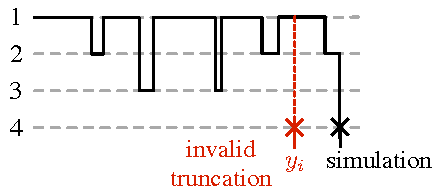
\includegraphics[width=0.35\textwidth]{Truncation}\end{center}
		\end{enumerate}
		
		\vspace{-0.5em}
		We propose two advances to remedy this.
		
		\vspace{0.5em}
		\textbf{a) Direct Conditional Sampling:} Rather than rejection sampling, which is susceptible to stalling, it is more desirable to sample $p(\mathrm{path\ \cdot} \,|\, \boldsymbol{\pi}, \mathbf{S}, Y \ge y_i)$ directly.  This requires the ability to sample from the conditional sojourn time density:
		\vspace{-0.5em}
		\[ p(\delta = \Delta \,|\, \boldsymbol{\pi}, \mathbf{S}, j(t), t, Y_i \ge y_i) \]
		
		\vspace{-0.5em}
		where $t$ is the current time and $j(t)$ the current state in the CTMC path being sampled.
		
		% \vspace{0.5em}
%		We have shown this can be calculated as:
%		\vspace{0.5em}
		\columnbreak
		
		This is nearly log-linear, though not log-concave.  Adaptive Rejection Metropolis Sampling (ARMS) has proven highly efficient.
		
		\vspace{0.5em}
		\textbf{b) Reverse Simulation:} For highly reliable systems, the starting state (full operation) is the most common.  Thus, by sampling in reverse from $y_i$ and truncating at 0 the commonality of state 1 becomes a major advantage and `invalid' proposals are rare.
		%\begin{center}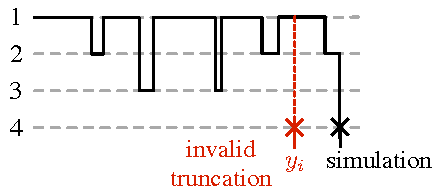
\includegraphics[width=0.35\textwidth]{Truncation}\end{center}
		
		\vspace{0.5em}
		This requires detailed balance to be satisfied.  Also, absorbing CTMCs don't necessarily reach stationarity, so selection of starting state must be made from the quasi-stationary distribution.
		
	\vspace{0.5em}
		\textbf{Speed Comparison:}
		
		\vspace{-1em}
		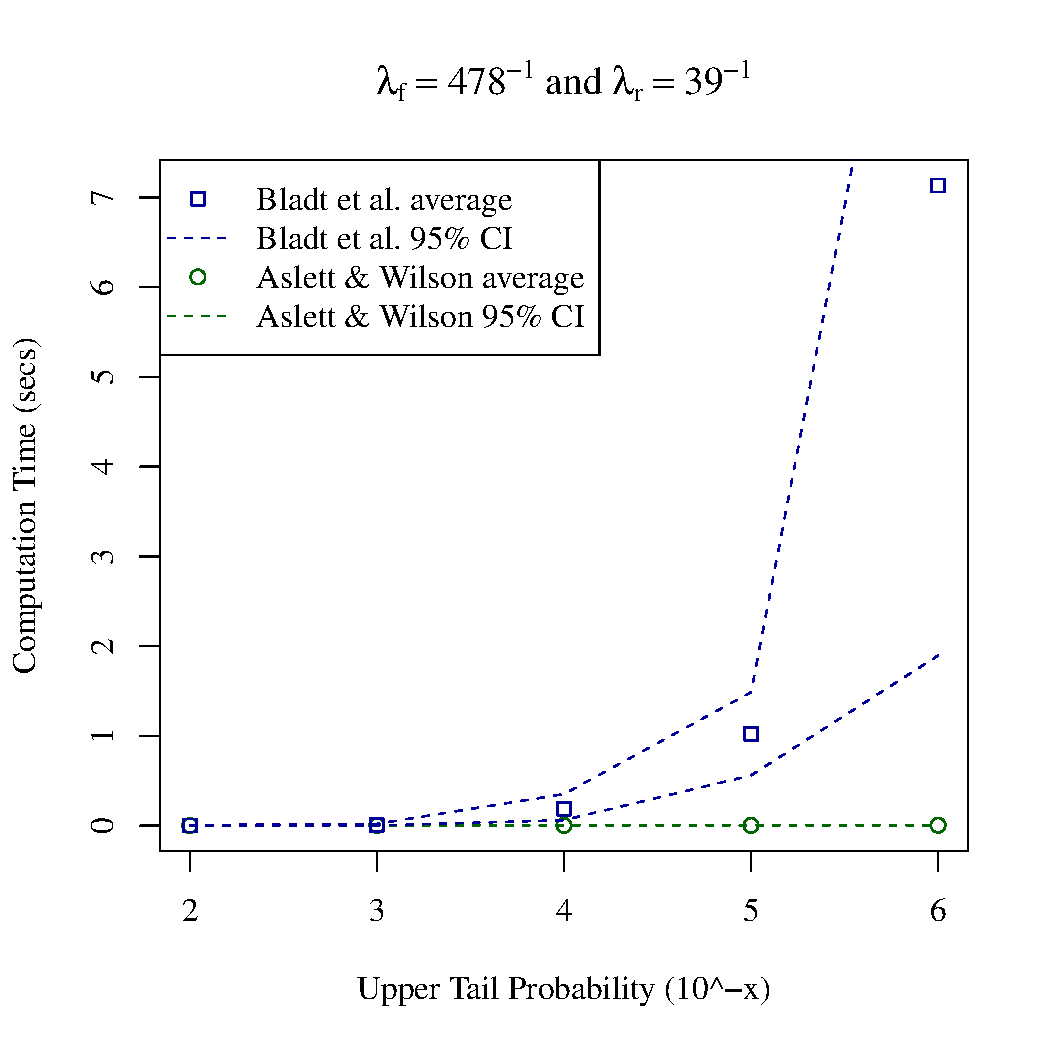
\includegraphics[width=0.5\textwidth]{SPEED}
	\end{multicols}
%	\vspace{-2em}
%	\[ = \frac{\displaystyle \left( \sum_{k=1}^n p(j(t+\Delta)=k \,|\, j(t), \mathbf{T}, t) p(Y_i \ge y_i-t-\Delta \,|\, \mathbf{T}) \right) p(\delta = \Delta \,|\, j(t), \mathbf{T}, t)}{\displaystyle p(Y_i \ge y_i \,|\, j(t), \mathbf{T}, t)} \]

}


\end{poster}%
\end{document}
